\documentclass{standalone}
\usepackage{tikz}

\begin{document}
        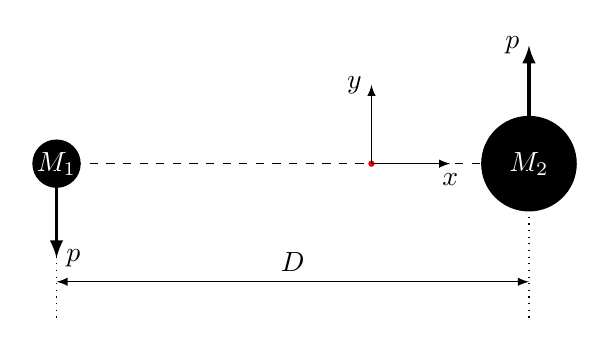
\begin{tikzpicture}
        	% line connecting BHs
        	\draw[dashed] (-4,0) -- (2,0);
        	\filldraw[color=white, fill=red] (0,0) circle (0.05);
        
        	% small BH
        	\filldraw[fill = black] (-4,0) circle (0.3);
        	\draw[very thick,-latex] (-4,0) -- (-4,-1.2);
        	\node[anchor=west] at (-4,-1.2) {$p$};
        	\node[color=white] at (-4,0) {$M_1$};
        	
        	% big BH
        	\filldraw[fill = black] (2,0) circle (0.6);
        	\draw[very thick,-latex] (2,0) -- (2,1.5);
        	\node[anchor=east] at (2,1.5) {$p$};
        	\node[color=white] at (2,0) {$M_2$};
        
        	% length
        	\draw[dotted] (2,0) -- (2,-2);
        	\draw[dotted] (-4,0) -- (-4,-2);
        	\draw[latex-latex] (-4,-1.5) -- (2,-1.5);
        	\node[anchor=south] at (-1,-1.5) {$D$};
        	
        	% axes
        	\draw[-latex] (0,0) -- (0,1);
        	\node [anchor=east] at (0,1) {$y$};
        	\draw[-latex] (0,0) -- (1,0);
        	\node[anchor=north] at (1,0) {$x$};
        \end{tikzpicture}
\end{document}